\begin{center}
\textbf{\Large Параболы}\\
\textit{8 класс}\\
\textit{05.07.17}
\end{center}

\begin{problems}
\item На рисунке изображены графики трёх квадратных трёчленов. Можно ли подобрать такие числа $a, b$ и $c$, чтобы это были графики трёхчленов $ax^2 + bx + c$, $bx^2 + cx + a$  и $cx^2 + ax + b$?
%http://www.problems.ru/view_problem_details_new.php?id=109457

\begin{center}
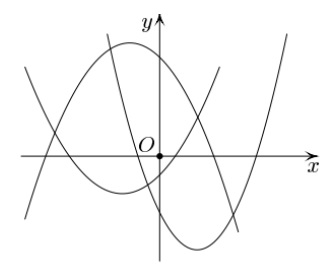
\includegraphics[scale=0.8]{simple/parabola.jpg}
\end{center}

\item Квадратный трехчлен $y = ax^2 + bx + c$  не имеет корней и $a + b + c > 0$.  Найдите знак коэффициента $c$.
%геометрическая интерпретация

\item Верно ли, что если $b > a + c > 0$, то квадратное уравнение $ax^2 + bx + c = 0$ имеет два корня?
%геометрическая интерпретация

\item Дан многочлен $P(x) = t^2 - 4t$. Доказать, что при любых $x \ge 1$ и $y \ge 1$ выполняется $P(x^2+y^2) \ge P(2xy)$. 

\item Существуют ли такие три квадратных трёхчлена, что каждый из них имеет хотя бы один корень, а сумма любых двух из них корней не имеет?

\item 

\item Приведенные квадратные трёхчлены $f(x)$ и $g(x)$ таковы, что уравнения  $f(g(x))\hm= 0$  и  $g(f(x)) = 0$  не имеют вещественных корней. Докажите, что хотя бы одно из уравнений  $f(f(x)) = 0$  и  $g(g(x)) = 0$  тоже не имеет вещественных корней.
\end{problems}